\documentclass{beamer}

\mode<presentation>
{
  \usetheme{boxes}      
  \usecolortheme{whale} 
  \usefonttheme{serif} 
  \setbeamertemplate{navigation symbols}{}
  \setbeamertemplate{caption}[numbered]
} 
\usepackage{tikz}
\setbeamercovered{highly dynamic}
\newcounter{saveenumi}
\newcommand{\seti}{\setcounter{saveenumi}{\value{enumi}}}
\newcommand{\conti}{\setcounter{enumi}{\value{saveenumi}}}
\renewcommand{\thefigure}{\thesection-\arabic{figure}}
\usetikzlibrary{shapes.geometric,calc,angles,positioning,intersections,quotes,decorations,babel,patterns,fit}
\usepackage{tkz-euclide}
\usetkzobj{all}
\usepackage[english]{babel}
\usepackage[utf8]{inputenc}
\usepackage[T1]{fontenc}
\usepackage{graphics}
\usepackage{standalone}
\usepackage{gensymb}
\usepackage{tikz}
\usetikzlibrary{shapes.geometric,calc,angles,positioning,intersections,quotes,decorations,babel,patterns,fit}
\usepackage{tkz-euclide}
\usetkzobj{all}
\usepackage{amsmath}
\title[Your Short Title]{Exercises}
\author{Durga Prasad}
\institute{}
\date{22 December 2019}
\begin{document}
\begin{frame}
  \titlepage
\end{frame}
\begin{frame}{Triangle exercise}
\begin{enumerate}
\item ABC and AMP are two right triangles, right
angled at B and M respectively. M lies on AC
and AB is extended to meet P. Prove that:
\seti
\begin{enumerate}
\item $\triangle{ABC} \sim \triangle{AMP}$
\item $\frac{CA}{PA}=\frac{BC}{MP}$
\end{enumerate}
\end{enumerate}
\textbf{Solution:}
\begin{figure}[!ht]
\resizebox{.4\linewidth}{!}
{
\begin{tikzpicture}[scale =2.5,>=stealth,point/.style = {draw, circle, fill = black, inner sep = 1pt},]
\node (C) at (4,3)[point,label=above :$C$] {};
\node (A) at (0,0)[point,label=below :$A$] {};
\node (B) at (4,0)[point,label=below :$B$] {};
\node (P) at (5,0)[point,label=below :$P$] {};
\node (M) at (3.2,2.4)[point,label=above :$\textbf{M}$] {};
\draw (A)--(B);
\draw (B)--(C);
\draw (C)--(A);
\draw (P)--(M);
\draw (B)--(P);
\tkzMarkRightAngle[fill=white!45,size=.3,mark=](C,B,A)
\tkzMarkRightAngle[fill=white!45,size=.3,mark=](A,M,P)
\end{tikzpicture}

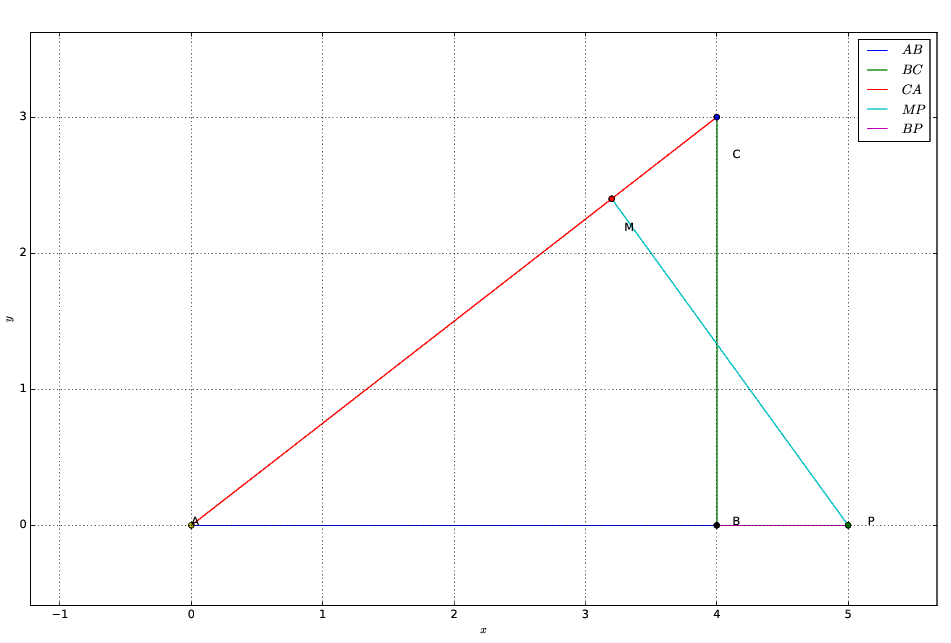
\includegraphics[scale=0.4]{./figs/triangle/tri.png}
}
\caption{right angled triangles}
\label{fig:foo}
\end{figure}
\end{frame}
\begin{frame}
From the above figure
\begin{align}
	\angle{CAB} =\angle{MAP} \\
	\angle{ABC} = \angle{AMP}
\end{align}
From 1 and 2
\begin{align}
\triangle{ABC} \sim \triangle{AMP}
\end{align}
\begin{itemize}
\item As correspondinng sides are proportional
$\frac{CA}{PA}=\frac{BC}{MP}=\frac{AB}{AM}$

\begin{center}
$\frac{CA}{PA}=\frac{BC}{MP}$
\end{center}
\end{itemize}
\end{frame}
\begin{frame}{Triangle construction}
\begin{enumerate}
\conti
\item In $\triangle{ABC}$ ,a=8,$\angle{B}=45\degree$ and c-b=3.5. Sketch $\triangle{ABC}$
\seti
\end{enumerate}
\textbf{Solution:}
\begin{figure}[!ht]
\resizebox{1\linewidth}{!}
{
\begin{tikzpicture}[scale =1,>=stealth,point/.style = {draw, circle, fill = black, inner sep = 2pt},]
\node (A) at (8.482904196010466,8.482904196010463)[point,label=above :$A$] {};
\node (B) at (0,0)[point,label=above :$B$] {};
\node (C) at (8,0)[point,label=below :$C$] {};
\draw[->,thick] (A) -- node[above] {$\textbf{c}$} (B) -- node[left] {$\textbf{a=8cm}$} (C) -- node[below,,xshift=1mm] {$\textbf{b}$} (A);
%Drawing and marking angles
\tkzMarkAngle[fill=white!45,size=.3,mark=](C,B,A)
\tkzLabelAngle[pos=0.65](A,B,C){$45$}
\end{tikzpicture}

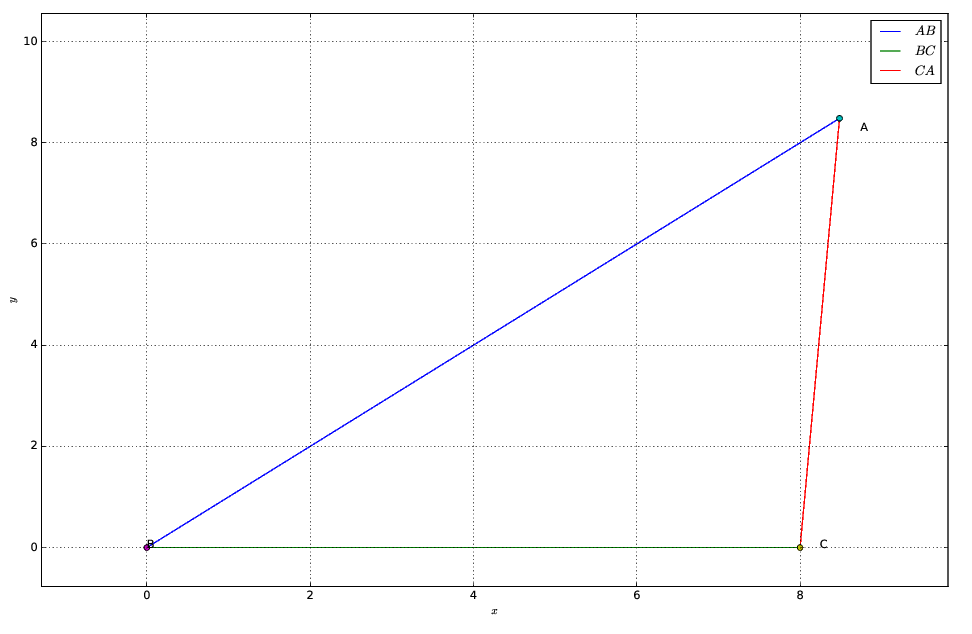
\includegraphics[scale=0.4]{./figs/triangle/constr.png}
}
\caption{Triangle with tikz and python }
\label{fig:foo}
\end{figure}
\end{frame}
\begin{frame}
Given a=8cm, c-b=k (k=3.5cm)
Apply cosine rule 
\begin{align*}
	\cos{(B)} = \frac{a^2+c^2-b^2}{2ac}\\
	\cos{(B)}= \frac{a^2+(b+k)^2-b^2}{2a(b+k)}\\
	2ab\cos{B}+2ak\cos{B}=a^2+k+2bk\\
	b=\frac{a^2 + k^2-2ak \cos{B} }{2a\cos{B}-2k}
\end{align*}
\begin{center}
b=8.49, c=11.99
\end{center}
\begin{itemize}
\item tikz code for above figure: \url{https://github.com/d-DP/Assignments/blob/master/figs/2.tex}
\item Python code for Figure 0-2:\url{https://github.com/d-DP/Assignments/blob/master/codes/2.py}\\
\end{itemize}
\end{frame}

\end{document}